\section{Nonlinear multi-observers}\label{ch:nonlinear-mos}
In this chapter the issues with MOs applied on nonlinear systems will be discussed. We will employ an MO on system \eqref{eqn:standard-system} which will be repeated here for clarity
\begin{equation*}
    \begin{split}
        \dot{x}(t) &= Ax(t) + Bu(t) + E\phi(x) \\
        y_i(t) &= C_ix(t) + Du(t) + v_i(t) + \tau_i(t) \quad i \in \mathcal{N} = \{1,2,\dots,N_O\}.
    \end{split}
\end{equation*}
First the observers will be extended with the aim of correctly observing the state of system \eqref{eqn:standard-system} when less then half of the sensors are under attack (the same boundary condition as discussed in Chapter \ref{ch:cmo}).

\subsection{Extending the state-estimates}
Let us extend the MO to also observe nonlinear systems as a single observer in Equation \eqref{eqn:nonlinear-single-observer}. First $H_x$ \eqref{eqn:Hx} has to be adapted to facilitate a nonlinearity $\phi$ as an input
\begin{equation}\label{eqn:Hy}
    H_y = 
    \begin{bmatrix}
        1 & 0 & 0 & \cdots & 0 \\
        -1 & 1 & 0 & \cdots & 0 \\
        -1 & -1 & 1 & \cdots & 0 \\
        \vdots & \vdots & \vdots & \ddots & \vdots \\
        -1 & -1 & -1 & \cdots & 1 
    \end{bmatrix}_{n_y \times n_y}.
\end{equation}
The multiplication $H_yy$ now gives all relative positions
\begin{equation*}
    H_yy =
    \begin{bmatrix}
        1 & 0 & 0 & \cdots & 0 \\
        -1 & 1 & 0 & \cdots & 0 \\
        -1 & -1 & 1 & \cdots & 0 \\
        \vdots & \vdots & \vdots & \ddots & \vdots \\
        -1 & -1 & -1 & \cdots & 1 
    \end{bmatrix}
    \begin{bmatrix}
        y_1 \\ y_2 \\ y_3 \\ \vdots \\ y_{n_y} \\
    \end{bmatrix}
    =
    \begin{bmatrix}
        y_1 \\
        y_2 - y_1 \\
        y_3 - y_2 - y_3 \\
        \vdots \\
        y_{n_y} - y_{n_y-1} - \cdots - y_2 - y_1 \\
    \end{bmatrix}.
\end{equation*}
Let us extend the observers as in Equations \eqref{eqn:cmo-single-J-observer}
\begin{equation}\label{eqn:nonlinear-mo}
    \begin{split}
        \dot{\hat{x}}_{j}^{\mcJ} &= (A + L_{j}^{\mcJ}C_{j}^{\mcJ})\hat{x}^{\mcJ}_{j} - L_{j}^JC_{j}^{\mcJ}x + Bu + E\phi(H_{y}y) - L_{j}^{\mcJ}(v_{j}^{\mcJ} + \tau_{j}^{\mcJ}) \\
        \dot{\hat{x}}_{p}^{\mcP} &= (A + L_{p}^{\mcP}C_{p}^{\mcP})\hat{x}^{\mcP}_{p} - L_{p}^JC_{p}^{\mcP}x + Bu + E\phi(H_{y}y) - L_{p}^{\mcP}(v_{p}^{\mcP} + \tau_{p}^{\mcP}),
    \end{split}
\end{equation}
where $j=1,2,\dots,N_J$ and $p=1,2,\dots,N_P$. The resulting observer in Equation \ref{eqn:nonlinear-mo} is analogous to the observer in \cite[Equation 5]{Chong2023MemoryAlgorithms}. In this case the nonlinearity is output dependent, the full $y$ is used as input and not the subset that corresponds to the the specific $p$ or $j$. This has some implications in the SSE context, where some $y_i$ are corrupted. If the $y_i$ that happens to be used by the nonlinearity $\phi(H_yy)$ is attacked, all state estimates become corrupted.

\begin{example}\label{ex:nonlinear-issue}
    Let us work through an example to clarify this issue, consider system \eqref{eqn:example-system} as defined in Example \ref{ex:system}, where we change $C$ to have $N_O=6$ outputs
    \begin{equation}\label{eqn:NL-ex-C-6out}
        C = 
        \begin{bmatrix}
            1 & 0 & 0 & 0 \\
            1 & 0 & 1 & 0 \\
            1 & 0 & 0 & 0 \\
            1 & 0 & 1 & 0 \\
            1 & 0 & 0 & 0 \\
            1 & 0 & 1 & 0 \\
        \end{bmatrix}.
    \end{equation}
    This means there are 3 copies of each sensor. The nonlinear spring as in Equation \eqref{eqn:nonlinear-spring} uses the spring constants and positions of each individual mass as input. Since we now have three copies of each position sensor we can select any combination of two sensors measuring a different position. Let us select the first two sensors, $y_1$ and $y_2$ by slicing the $H_y$ matrix \eqref{eqn:Hy}
    \begin{equation*}
        H_y = 
        \begin{bmatrix}
            1 & 0 & 0 & 0 & 0 & 0 \\
            -1 & 1 & 0 & 0 & 0 & 0 \\
        \end{bmatrix}
    \end{equation*}
    We now construct
    \begin{equation}\label{eqn:NL-ex-phi-6out}
        \phi(H_yy) = 
        \begin{bmatrix}
            F^{NL}_s(y_1) \\ F^{NL}_s(y_2 - y_1) \\
        \end{bmatrix},
    \end{equation}
    Which leads to the following $E$ matrix
    \begin{equation}\label{eqn:NL-ex-E-6out}
        E =
        \begin{bmatrix}
            0 & 0 \\
            -1 & 1 \\
            0 & 0 \\
            0 & -1 \\
        \end{bmatrix}.
    \end{equation}
    Figure \ref{fig:nonlinear-functional} displays a scenario where $\mathcal{M}=\{3,6\}$, so outputs $3$ and $6$ are under attack, with the attack signal $\tau_k=t,k \in \mathcal{M}$ The MO works as expected and provides a correct state estimate. The $\phi(H_yy)$ provides a correct value for all $t \geq 0$.
    \begin{figure}[H]
        \centering
        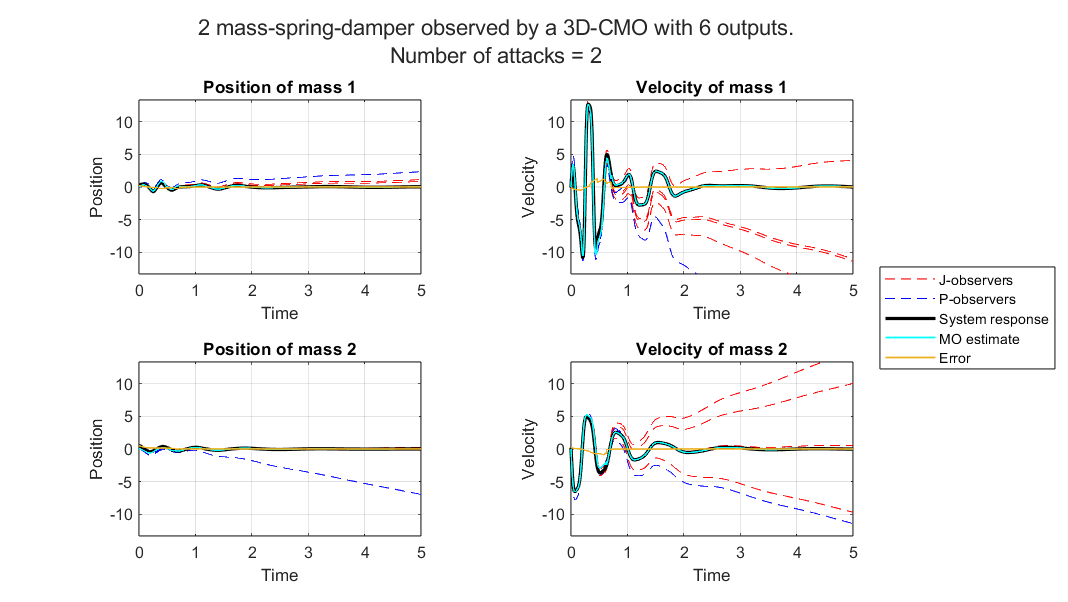
\includegraphics[width=\linewidth]{report/Figures/nonlinear_functional.png}
        \caption{Nonlinear double mass-spring-damper model with outputs $3$ and $6$ under attack.}
        \label{fig:nonlinear-functional}
    \end{figure}
    Figure \ref{fig:nonlinear-not-functional} shows a scenario where $\mathcal{M}=\{1,4\}$. Or in other words, outputs $1$ and $4$ are under attack. The attack signal is the same as in the previous case, $\tau_k=t,k \in \mathcal{M}$. All state estimates fail in this case, because $\phi(H_yy)$ uses an attacked output.

    \begin{figure}[H]
        \centering
        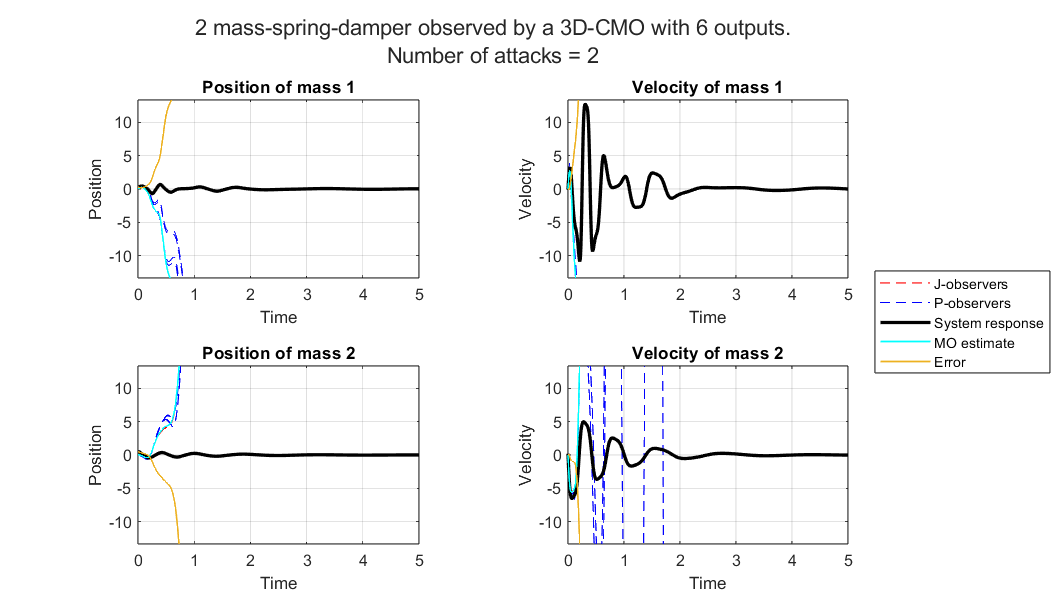
\includegraphics[width=\linewidth]{report/Figures/nonlinear_not_functional.png}
        \caption{Nonlinear double mass-spring-damper model with outputs $1$ and $4$ under attack.}
        \label{fig:nonlinear-not-functional}
    \end{figure}
\end{example}

Both Figures \ref{fig:nonlinear-functional} and \ref{fig:nonlinear-not-functional} show the result of a 3D-CMO, the result on an SSMO is the same. Not surprising, since they realize the same set of observers.

\subsection{Investigating the nonlinear issue}\label{subsec:investigating-nonlinear-issue}
As discussed in Example \ref{ex:nonlinear-issue} the issue arises because the observers' nonlinear extension does not employ any intelligent logic in choosing which outputs are used to calculate the nonlinear contribution. The nonlinearity $\phi(H_yy)$ should either 'know' which $y_i$ are corrupted and avoid them, which is contradictory with the demands of SSE. Or it should be able to provide a correct state estimate even with an unknown subset of sensors under attack. Let us now discuss the implications and difficulties of this issue for both the 3D-CMO and the SSMO, we will not consider the 2D-CMO in this section. 

Let us start with the SSMO, the shared state is calculated as in Equation \eqref{eqn:ssmo-z} which we repeat for readability
\begin{equation*}
    \dot{z} = \mathbf{A}z + \mathbf{B}\eta, \quad \eta = 
    \begin{bmatrix}
        u \\ y
    \end{bmatrix}.
\end{equation*}
The nonlinearity no longer appears in this structure, since it is taken into account during construction of the shared $\mathbf{B}$ matrix. The input to the nonlinear function $\phi(H_yy)$ is also 'hidden' behind the shared state. We cannot try different combinations of sensors $y_i$ because we only calculate a single state $z$, which uses a single external input $\eta$ with the full output $y$.

We now continue with the 3D-CMO, which has more control over each individual state estimate $\hat{x}^{\mcJ/\mcP}_{j/p}$. Since every observer is calculated separately, a different nonlinear contribution can be used for every observer.
\begin{equation}\label{eqn:ext-NL-observer}
    \begin{split}
        \dot{\hat{x}}_{j}^{\mcJ} &= (A + L_{j}^{\mcJ}C_{j}^{\mcJ})\hat{x}^{\mcJ}_{j} - L_{j}^JC_{j}^{\mcJ}x + Bu + E\phi(H^{\mcJ}_yy^{\mcJ}_{j}) - L_{j}^{\mcJ}(v_{j}^{\mcJ} + \tau_{j}^{\mcJ}) \\
        \dot{\hat{x}}_{p}^{\mcP} &= (A + L_{p}^{\mcP}C_{p}^{\mcP})\hat{x}^{\mcP}_{p} - L_{p}^JC_{p}^{\mcP}x + Bu + E\phi(H^{\mcP}_yy^{\mcP}_{p}) - L_{p}^{\mcP}(v_{p}^{\mcP} + \tau_{p}^{\mcP}),
    \end{split}
\end{equation}
where
\begin{equation*}
    H^{\mcJ}_y = 
    \begin{bmatrix}
        1 & 0 & 0 & \cdots & 0 & \cdots & 0 \\
        -1 & 1 & 0 & \cdots & 0 & \cdots & 0 \\
        -1 & -1 & 1 & \cdots & 0 & \cdots & 0 \\
        \vdots & \vdots & \vdots & \ddots & \vdots &  & \vdots \\
        -1 & -1 & -1 & \cdots & 1 & \cdots & 0 \\
    \end{bmatrix}_{n_{\phi} \times J}, \quad
    H^{\mcP}_y = 
    \begin{bmatrix}
        1 & 0 & 0 & \cdots & 0 & \cdots & 0 \\
        -1 & 1 & 0 & \cdots & 0 & \cdots & 0 \\
        -1 & -1 & 1 & \cdots & 0 & \cdots & 0 \\
        \vdots & \vdots & \vdots & \ddots & \vdots &  & \vdots \\
        -1 & -1 & -1 & \cdots & 1 & \cdots & 0 \\
    \end{bmatrix}_{P \times n_y}
\end{equation*}
The nonlinear contribution $E\phi(H^{\mcJ/\mcP}_yy^{\mcJ/\mcP}_{j/p})$ uses the subset $j$ or $p$ as input to the function $\phi(H_yy)$. Let us work out two examples that clarify some of the implications this extended 3D-CMO has. We start with an example that investigates a system where $\phi(H_yy)$ is dependent only on one measured state variable.

\begin{example}\label{ex:single-mass-nonlinear-example}
    Consider the system as in Equation \eqref{eqn:standard-system} with system matrices
    \begin{equation*}
        A =
        \begin{bmatrix}
            0 & 1 \\ -15 & -2 \\
        \end{bmatrix}, \quad
        B =
        \begin{bmatrix}
            0 \\ 1 \\
        \end{bmatrix}, \quad
        C = 
        \begin{bmatrix}
            1 & 0 \\ 1 & 0 \\ 1 & 0 \\ 1 & 0 \\ 1 & 0 \\
        \end{bmatrix}, \quad
        D = 0, \quad
        E =
        \begin{bmatrix}
            0 \\ -1 \\
        \end{bmatrix},   
    \end{equation*}
    as derived from the general mass-spring-damper described in Chapter \ref{ch:system-definition}.  The nonlinearity looks like
    \begin{equation*}
        \begin{split}
            \phi(H^{\mcJ}_{y}y^{\mcJ}_{y}) &= F^{NL}_s(y^{\mcJ}_{1}) \\
            \phi(H^{\mcP}_{y}y^{\mcP}_{y}) &= F^{NL}_s(y^{\mcP}_{1}) \\
        \end{split}        
    \end{equation*} 
    where
    \begin{equation*}
        H^{\mcJ}_{y} =
        \begin{bmatrix}
            1 & 0 & 0
        \end{bmatrix}, 
        \quad H^{\mcP}_{y} = 1.
    \end{equation*}
    The system has $N_O=5$ outputs, let us attack $N_M=2$ of those outputs. $\mathcal{M}=\{2,4\}$, so outputs $2$ and $4$ are under attack. Again the attack signal $\tau_k=t,k \in \mathcal{M}$ is used. Figure \ref{fig:single-nonlinear-functional} shows the result of such an attack, the MO successfully estimates the state and the error approaches zero. 
    \begin{figure}[H]
        \centering
        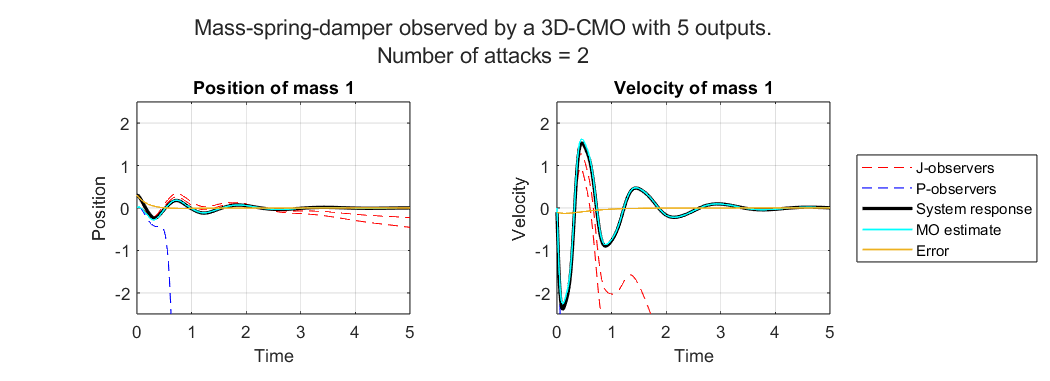
\includegraphics[width=\linewidth]{report/Figures/single-nonnlinear-functional.png}
        \caption{Single nonlinear mass-spring-damper with outputs $2$ and $4$ under attack.}
        \label{fig:single-nonlinear-functional}
    \end{figure}
    In this scenario the MO functions because all sensors measure the same variable, the position of the first (and only) mass. So the combination $j=\{1,3,5\}$ provides a successful state estimate because $F^{NL}_s(y_1) = F^{NL}_s(y_3) = F^{NL}_s(y_5)$ and since the nonlinearities equal
    \begin{equation*}
        \begin{split}
            \phi \left( H^{\mcJ}_{y}
            \begin{bmatrix}
                y_1 \\ y_3 \\ y_5
            \end{bmatrix} \right) &= \phi(y_1) = F^{NL}_s(y_1) \\       \phi \left( H^{\mcP}_{y}y_1 \right) &= \phi(y_1) = F^{NL}_s(y_1) \\
            \phi \left( H^{\mcP}_{y}y_3 \right) &= \phi(y_3) = F^{NL}_s(y_3) \\
            \phi \left( H^{\mcP}_{y}y_5 \right) &= \phi(y_5) = F^{NL}_s(y_5). \\
        \end{split}
    \end{equation*} 
\end{example}
Let us now investigate a scenario where the nonlinearity $\phi(y)$ depends on multiple measured state variables.

\begin{example}\label{ex:ext-NL-double-mass}
    Now, consider the same system \eqref{eqn:example-system} as in Example \ref{ex:system}, where $C$ is changed to have $N_O=5$
    \begin{equation*}
        C = 
        \begin{bmatrix}
            1 & 0 & 0 & 0 \\
            1 & 0 & 1 & 0 \\
            1 & 0 & 0 & 0 \\
            1 & 0 & 1 & 0 \\
            1 & 0 & 0 & 0 \\
        \end{bmatrix}.
    \end{equation*}
    The $H$ matrices are again sliced from \eqref{eqn:Hy} as
    \begin{equation*}
        H^{\mcJ}_y =
        \begin{bmatrix}
            1 & 0 & 0 \\
            -1 & 1 & 0 \\
        \end{bmatrix}, \quad
        H^{\mcP}_y = 1     
    \end{equation*}
    which leads to
    \begin{equation*}
        \phi(H^{\mcJ}_yy^{\mcJ}_j) =
        \begin{bmatrix}
            F^{NL}_s({y^{\mcJ}_j}_1) \\
            F^{NL}_s({y^{\mcJ}_j}_2 - {y^{\mcJ}_j}_1)
        \end{bmatrix}, \quad
        y^{\mcJ}_j=
        \begin{bmatrix}
            {y^{\mcJ}_j}_1 \\ {y^{\mcJ}_j}_2 \\ {y^{\mcJ}_j}_3 \\
        \end{bmatrix}
    \end{equation*}
    and $E$ is as in Equation \eqref{eqn:NL-ex-E-6out}. Let us now choose $N_M=2$ in order to still satisfy the $N_O>2N_M$ requirement. Where we specify $\mathcal{M}$ as $\{2,4\}$, note that now all copies of the sensor measuring the position of mass 2 are attacked. Figure \ref{fig:extended_nonlinear_not_functional} shows that the error $\hat{x}-x$ still approaches $0$ as $t$ increases. But the estimates, especially of the velocities, do not look to be tracking the true state correctly.
    \begin{figure}[H]
        \centering
        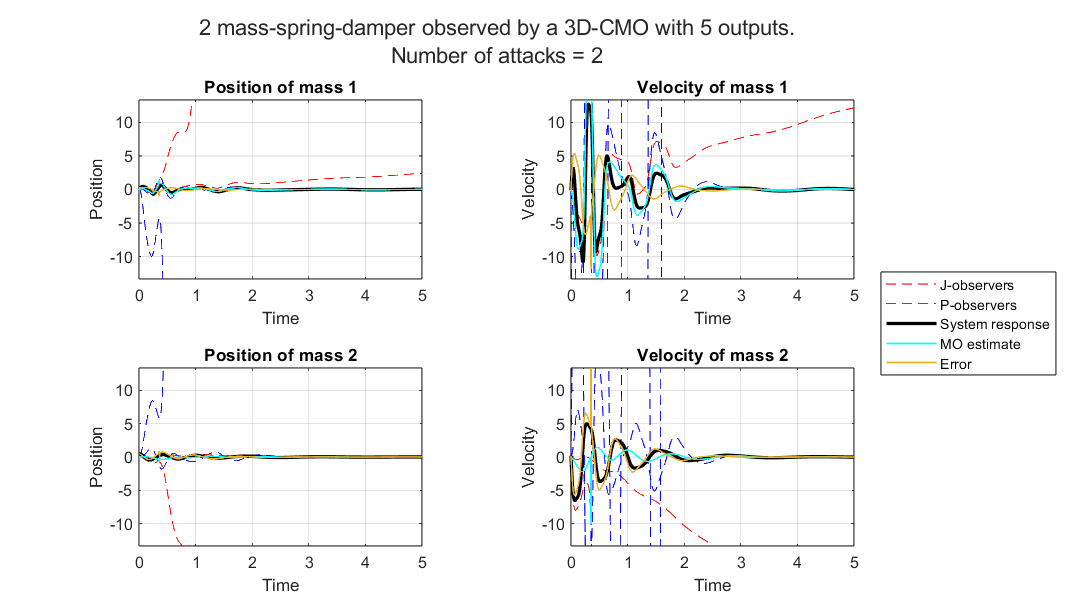
\includegraphics[width=\linewidth]{report/Figures/extended_nonlinear_not_functional.png}
        \caption{Double nonlinear mass-spring-damper with outputs 2 and 4 under attack.}
        \label{fig:extended_nonlinear_not_functional}
    \end{figure}
    Let us now expand the number of outputs to $N_O=6$, and use the exact same system as in Equations \eqref{eqn:NL-ex-C-6out},\eqref{eqn:NL-ex-E-6out} and \eqref{eqn:NL-ex-phi-6out} as in Example \ref{ex:nonlinear-issue}. We now use the observer as in Equation \eqref{eqn:ext-NL-observer} and attack the system with the attack signal $\tau_k=t,k \in \mathcal{M},\mathcal{M}=\{4,6\}$ \textcolor{red}{ugly}.
    \begin{figure}[H]
        \centering
        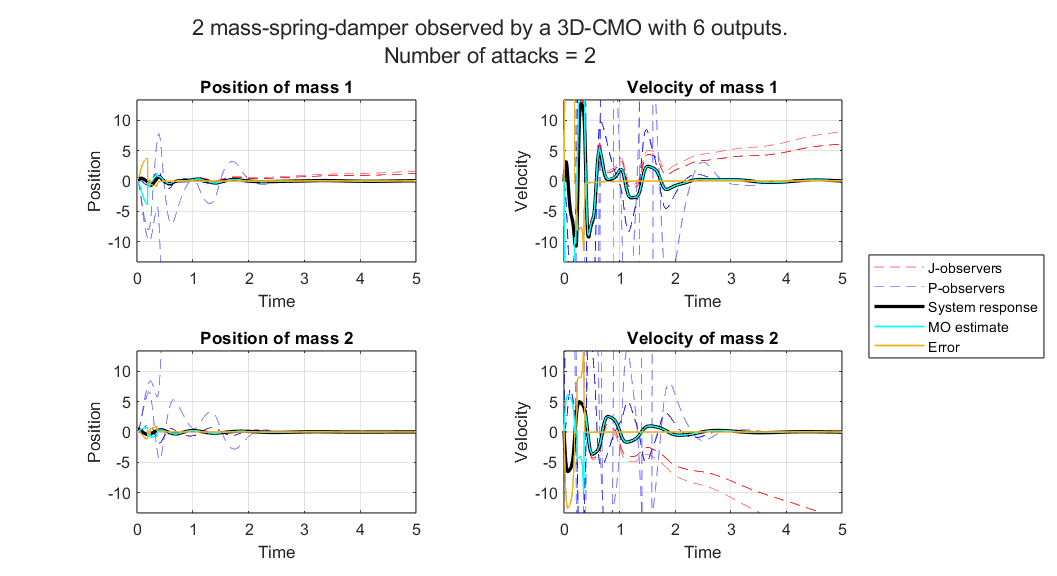
\includegraphics[width=\linewidth]{report/Figures/extended-nonlinear-functional.png}
        \caption{Double mass-spring-damper with outputs $4$ and $6$ under attack.}
        \label{fig:extended-nonlinear-functional}
    \end{figure}
    The state estimates in Figure \ref{fig:extended-nonlinear-functional} look to be tracking the true state much better. The MO now functions correctly because the state estimate using $j=\{1,2,3,5\}$ has the uncorrupted outputs $1$ and $2$ as input to $\phi(y)$ as in Equation \eqref{eqn:NL-ex-phi-6out}.
\end{example}
The attacked outputs in Example \ref{ex:ext-NL-double-mass} have, of course, been carefully chosen to provide the correct results. Had we attacked outputs $2$ and $4$ in the $N_O=6$ case, no correct state estimate could have been provided. This happens because the nonlinearity $\phi(y)$ in the example takes the first two entries of $y^{\mcJ/\mcP}_{j/p}$ irrespective of what the sensor measures. So if outputs $2$ and $4$ are attacked, even the fully uncorrupted set of outputs $j=\{1,3,5,6\}$ does not provide a correct state estimate. Because $\phi(y)$ is only considers outputs $1$ and $3$ in this state estimate. If the list would have been ordered as $\{1,6,3,5\}$ the observer would provide a correct estimate. However, the selection procedure would not work. During the final estimate selection procedure as described in subsection \ref{subsec:estimate-selection}. All estimates constructed with $p \in j$ are compared against the estimate constructed with $j$. We now encounter the same obstacle as before: for all subsets $|p| < |j|, p \subset j$, some do not contain any sensor measuring the position of the second mass. Those estimates will suffer the same fate as the $J$-observers discussed before and provide a wrong state estimate. Even though its 'parent' estimate is correct.

\subsection{Addressing the nonlinear issue}
Let us develop a new approach in order to tackle this issue. Consider system \eqref{eqn:standard-system} with outputs
\begin{equation*}
    y_i, i \in \{1,2,\dots,N_O\}.
\end{equation*}
We now define \textit{aggregate sensors} that combine multiple $y_i$ as
\begin{equation}
    \nu_g = 
    \begin{bmatrix}
        y_{g_1} \\ y_{g_2} \\ \vdots \\ y_{g_{|g|}} \\
    \end{bmatrix}
    , \quad g \subset \{1,2,\dots,N_O\} \quad \text{and} \quad 1 < n_g < N_O,
\end{equation}
where $n_g=|g|$. As discovered in subsection \ref{subsec:investigating-nonlinear-issue}, the order in which sensors appear should be standardized between all aggregate sensors $\nu_g$. For simplicity, the same order as in which variables are required in the nonlinearity will be used.

\begin{example}\label{ex:aggregate-sensors}
    Consider system \eqref{eqn:example-system} as in Example \ref{ex:system} with $C$ as in equation \eqref{eqn:NL-ex-C-6out} and $\phi(y)$ as in equation \eqref{eqn:NL-ex-phi-6out}. The nonlinearity expects a measurement of $x_1$ and a measurement of $x_3$, which is constructed by subtracting a measurement of absolute position of the first mass from a measurement of the absolute position of the second mass. This implies $|g|=n_{\phi}=2$, where $g$ could be $\{1,2\},\{3,4\}$ or $\{5,6\}$. Aggregate sensors made up of sensor groups that 'neighbour' each other in the matrix $C$ will be called \textit{strict aggregate sensors}.

    We can also be less strict on the values $g$ can take. For example, in addition to the strict combinations $g$ could also be $\{1,4\},\{1,6\},\{3,2\},\{3,6\},\{5,2\}$ or $\{5,4\}$. Such aggregate sensors will be called \textit{loose aggregate sensors}.
\end{example}

With these aggregate sensors we now construct the state estimates as we have done before, let us start with creating the $J$ and $P$-observers. We follow the same procedure as described in subsection \ref{subsec:state-estimates}, now we only consider the aggregate sensors $\nu$ as outputs. In Example \eqref{ex:aggregate-sensors} the de facto number of outputs is halved, to $N_O=3$ outputs. For MOs employing strict aggregate sensor grouping the total number of sensors or rows of $C$, in this case $6$, is denoted as $N_S$. In general
\begin{equation*}
    N_O = \frac{N_S}{n_{\phi}}, \quad N_O \in \mathbb{N} \implies N_S = \alpha n_{\phi}, \quad \alpha \in \mathbb{N}
\end{equation*}
so the number of sensors must equal a multiple of the number of nonlinearities. We can now construct an MO as in Equation \eqref{eqn:ext-NL-observer}, with some extra requirements on $j$ and $p$. Since observers are now constructed with combinations of $\nu_i,i=1,2,\dots,N_O$, we cannot simply take every possible combination of the set $\{1,2,\dots,N_S\}$ with sizes $J$ and $P$ respectively. 

Let us start by discussing the number of attacks $N_M$, this number indicates the amount of sensors that are under attack. Those individual sensors could be in the same aggregate sensor. We will assume the worst case, all attacked sensors are in a different aggregate sensor. Let us define $N_A$ as the number of attacked aggregate sensors. The sizes of each $J$ and $P$-observer are
\begin{equation}\label{eqn:AMO-observer-sizes}
    \begin{split}
        J_{agg}&=N_O-N_A, \quad P_{agg}=1 \\
        J_{ind} &= n_{\phi}J_{agg}, \quad P_{ind} = n_{\phi}P_{agg},
    \end{split}
\end{equation}
where the subscript $agg$ denotes the number of aggregate sensors and the subscript $ind$ denotes the amount of individual sensors. The condition as in Equation \eqref{eqn:MO-size-requirement} that $N_O>2N_M$ still holds. Equation \eqref{eqn:AMO-observer-sizes} implies that more sensors are required as compared to a linear MO. 
\begin{equation*}
    N_O > 2N_M \implies N_O \geq 2N_M + 1 \implies N_S \geq (2N_M + 1)n_{\phi}
\end{equation*}
which implies that the number of sensors required is $n_{\phi}$ times larger. We now construct all $J$-observers by creating all combinations of $\nu_i,i=1,2,\dots,N_O$ and all $P$-observers use a single $\nu_i$, which results in the following number of observers
\begin{equation*}
    N_J = \binom{N_O}{J_{agg}}, \quad N_P = \binom{N_O}{P_{agg}}.
\end{equation*}


\begin{example}\label{ex:strict-aggregate}
    Consider the system as in Example \ref{ex:nonlinear-issue} described by Equations \eqref{eqn:example-system},\eqref{eqn:NL-ex-E-6out}. With 
    \begin{equation*}
        C =
        \begin{bmatrix}
            \Tilde{C}^{T} &
            \Tilde{C}^{T} &
            \Tilde{C}^{T} &
            \Tilde{C}^{T} &
            \Tilde{C}^{T} 
        \end{bmatrix}^{T}, \quad
        \Tilde{C} = 
        \begin{bmatrix}
            1 & 0 & 0 & 0 \\
            1 & 0 & 1 & 0 \\
        \end{bmatrix}
    \end{equation*}
    and 
    \begin{equation*}
        \phi(H^{\mcJ}y^{\mcJ}_j) =
        \begin{bmatrix}
            F^{NL}_s({y^{\mcJ}_j}_{1}) \\
            F^{NL}_s({y^{\mcJ}_j}_{2} - {y^{\mcJ}_j}_1)
        \end{bmatrix} 
        \quad \text{and} \quad
        \phi(H^{\mcP}y^{\mcP}_p) =
        \begin{bmatrix}
            F^{NL}_s({y^{\mcP}_p}_{1}) \\
            F^{NL}_s({y^{\mcP}_p}_{2} - {y^{\mcP}_p}_{2})
        \end{bmatrix},
    \end{equation*}
    where
    \begin{equation*}
        \begin{split}
            H^{\mcJ}_y &=
            \begin{bmatrix}
                1 & 0 & 0 & 0 & 0 & 0 \\
                -1 & 1 & 0 & 0 & 0 & 0 \\
            \end{bmatrix}, \quad 
            H^{\mcP}_1 =
            \begin{bmatrix}
                1 & 0 \\
                -1 & 1 \\
            \end{bmatrix}.
        \end{split}
    \end{equation*}
    We apply strict aggregate sensor grouping on the $N_S=10$ sensors gives the following aggregate sensors
    \begin{equation*}
        \nu_1 = 
        \begin{bmatrix}
            y_1 \\ y_2
        \end{bmatrix}, \quad
        \nu_2 = 
        \begin{bmatrix}
            y_3 \\ y_4
        \end{bmatrix}, \quad
        \nu_3 = 
        \begin{bmatrix}
            y_5 \\ y_6
        \end{bmatrix}, \quad
        \nu_4 =
        \begin{bmatrix}
            y_7 \\ y_8
        \end{bmatrix}, \quad
        \nu_5 = 
        \begin{bmatrix}
            y_9 \\ y_{10}
        \end{bmatrix}.
    \end{equation*}
    This system has $N_O=5$ and can thus handle $2$ attacks which implies that $N_A=2$. So, the $J$-observers use $J_{agg}=3$ aggregate sensors. Figure \ref{fig:aggregate-functional} shows such a scenario, where the MO behaves as expected.

    \begin{figure}[H]
        \centering
        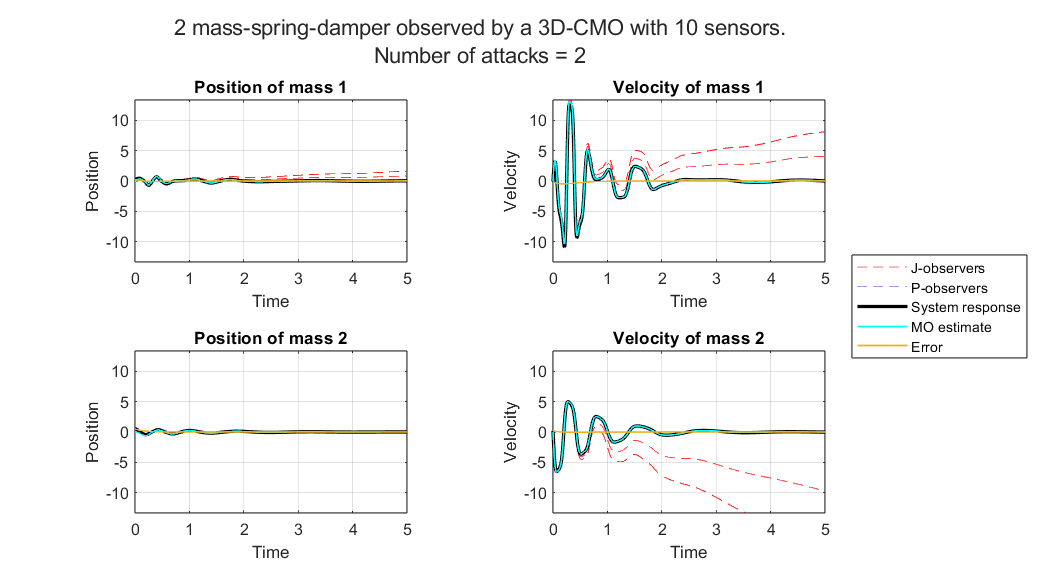
\includegraphics[width=\linewidth]{report/Figures/aggregate-nonlinear-10o2a.png}
        \caption{A double mass-spring-damper with aggregate sensors, outputs 4 and 6 are under attack}
        \label{fig:aggregate-functional}
    \end{figure}
    
\end{example}
Let us define the concept of an MO being \textit{robust to an attack}, the MO in Example \ref{ex:aggregate-sensors} is robust to any attack with $N_M=2$. It is also robust to the attack where $\mathcal{M}=\{1,2,3\}$, since only 2 of 5 aggregate sensors are attacked. Such an attack corrupts less than half of all aggregate sensors. The number of aggregate sensors attacked will be denoted as $N_A$. In general a SAMO, strict agrregate multi-observer, is robust to an attack when
\begin{equation}\label{eqn:robust-to-an-attack-SAMO}
    N_O > 2N_A.
\end{equation}
Thus $N_A$ decides whether an MO with $N_O$ outputs is robust to the attack. For the system in Example \ref{ex:aggregate-sensors} with $N_M$ attacks, $N_A$ could be equal to $1$ or $2$. That always satisfies the condition in Equation \eqref{eqn:robust-to-an-attack-SAMO}. When $N_M=3$ or $N_M=4$, the MO is robust to some attacks. The worst case attack would be to attack as many copies of a single sensor.
\begin{example}\label{ex:SAMO-attack}
    Consider the same system as in Example \ref{ex:strict-aggregate}, let us now perform the following attack: $\mathcal{M}=\{1,3,5\}$ where $\tau_i=t,i\in\mathcal{M}$. Figure \ref{fig:SAMO-attack} shows this scenario, the SAMO is clearly not robust with respect to this attack. Not strange considering $N_O< 2N_A$.

    \begin{figure}[H]
        \centering
        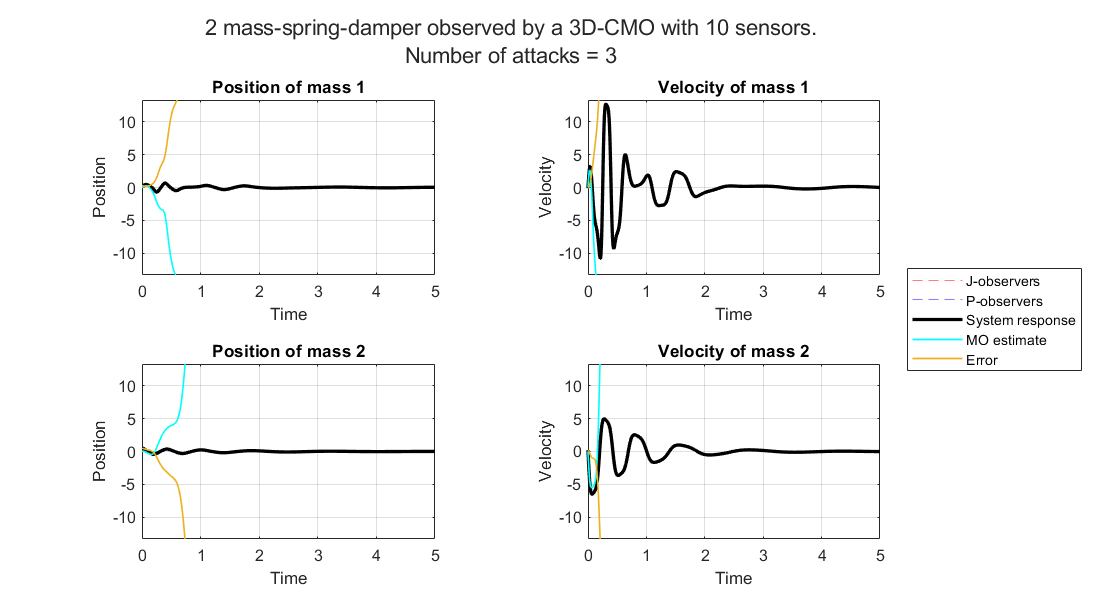
\includegraphics[width=\linewidth]{report/Figures/SAMO-attack-not-robust.png}   
        \caption{SAMO with $N_S=10$ and $n_{\phi}$, where outputs 1,3 and 5 are under attack.}
        \label{fig:SAMO-attack}
    \end{figure}
\end{example}
So a MO is only robust to some attacks that target 3 sensors. Let us now work out the probability of the system being robust to an attack targetting 3 randomly picked sensors.

\begin{example}\label{ex:SAMO-probability}
    Consider the system as in Example \ref{ex:SAMO-attack}, let us pick $N_M=3$ random sensors out of the $N_S=10$. We first calculate the probability of picking $3$ sensors that end up being members of two distinct aggregate sensors
    \begin{equation*}
        p(N_A=2) = \frac{\displaystyle 5 \cdot 8}{\displaystyle  \binom{10}{3}} = \frac{40}{120} = 0.333,
    \end{equation*}
    where the numerator is the number of possible combinations with $N_A=2$ and the denominator is the total number of combinations. Let us further explain the rationale behind the $5 \cdot 8 = 40$ combinations in the numerator. Imagine that sensors $\{1,2\}$ are under attack, there are now $8$ more sensors to choose from. So, this gives $8$ combinations for a single sensor group. Since there are $5$ groups in this scenario the number of combinations is $40$. 
    
    Since there are only two options ($N_A = 2$ or $N_A=3$), $p(N_A=3)=1-p(N_A=2)$. However, we will work out $p(N_A=3)$ as well in order to get some insight into that probability
    \begin{equation*}
        p(N_A=3) = \frac{\displaystyle \binom{5}{3}2^3}{\displaystyle \binom{10}{3}} = \frac{80}{120} = 0.667
    \end{equation*}
    The denominator remains the same, unsurprising since the number of combinations of 3 out of 10 does not change. The logic behind the numerator requires some more explanation. Imagine we have selected any $3$ aggregate sensors, we can now choose one of two possible individual sensors from each of these aggregate sensors. Which leads to $2\cdot2\cdot2=8$ possible choices. Since $\binom{5}{3}=10$ combinations of aggregate sensors can be made, there are $80$ possibilities where $N_A=3$. This means that if an attacker attacks $3$ random outputs, the probability is $0.333$ that the SAMO is robust to the attack.
\end{example}
We now expand the concept of an MO being robust to an attack, the MO in Example \ref{ex:SAMO-probability} is \textit{fully robust to 2 attacks}. A system is fully robust to $N_M$ attacks if there is zero probability that $2N_A \geq N_O$ for an attack targetting $N_M$ sensors. The same MO is only \textit{partially robust to 3 attacks}. Let us define a \textit{robustness score} that indicates probability that an MO is robust to an attack targetting $N_M$ randomly selected sensors
\begin{equation}\label{eqn:robustness-score}
    r_{N_M} = p(2N_A < N_O | N_M).
\end{equation}
A robustness score of 1 for a certain $N_M$ is equal to a system being fully robust to $N_M$ attacks and a robustness score of 0 indicates that any attack targetting $N_M$ sensors will be successful. Instead of calculating the probabilities analytically as in Example \ref{ex:SAMO-probability}, the Matlab script in Appendix \ref{ap:matlab-code-ch7} loops over each possible attack and calculates $N_A$. From there the probabilities are derived by taking the fraction of of the total number of combinations. 

We now aim to compare LAMOs (loose aggregate multi-observers) to SAMOs in terms of robustness scores. First, LAMO observer sizes need to be investigated, since the worst case assumption for SAMOs that $N_A=N_M$ does not apply to LAMOs. It was only possible because every individual sensor only appeared in one aggregate sensor. 

\begin{example}\label{ex:LAMO-attack}
    Let us illustrate this difference using an example. Consider the same system as in Example \ref{ex:SAMO-probability}, we now create loose aggregate sensors instead of strict aggregate sensors
    \begin{equation}
        \nu_1 = 
        \begin{bmatrix}
            y_1 \\ y_2
        \end{bmatrix}, \quad
        \nu_2 = 
        \begin{bmatrix}
            y_1 \\ y_4
        \end{bmatrix}, \quad
        \nu_3 = 
        \begin{bmatrix}
            y_1 \\ y_6
        \end{bmatrix}, \quad
        \nu_4 =
        \begin{bmatrix}
            y_3 \\ y_2
        \end{bmatrix}, \quad \cdots \quad
        \nu_{24} = 
        \begin{bmatrix}
            y_9 \\ y_{8}
        \end{bmatrix}, \quad
        \nu_{25} =
        \begin{bmatrix}
            y_9 \\ y_{10}
        \end{bmatrix}.
    \end{equation}
    The 25 aggregate sensors imply that $N_O=25$ and thus, according to the robustness condition in Equation \eqref{eqn:robust-to-an-attack-SAMO}, would require at least $13$ aggregate sensors to be attacked. Every single sensor $y_i,i=1,2,\dots,10$ appears in 5 aggregate sensors $\nu_k,k=1,2,\dots,25$. This implies that the MO is not robust against an attack that corrupts 3 sensors measuring the same variable, for example, $y_1, y_3$ and $y_5$. Since such an attack corrupts $15$ aggregate sensors.
\end{example}
So the assumption $N_A=N_M$ does not hold for a LAMO, and thus the size of a LAMO should be decided in another way. In order choose a good number of aggregate sensors for each $J$-observer, the sizes of LAMOs should be worked out. Let us consider a system with $N_S$ sensors and $n_{\phi}$ nonlinearities, this implies that there are $N_S/n_{\phi}$ sensors measuring each nonlinear variable. Since we use all combinations between sensors measuring a different variable, there are
\begin{equation}\label{eqn:num-N_O-LAMO}
    N_O = \left( \frac{N_S}{n_{\phi}} \right) ^{n_{\phi}}
\end{equation}
aggregate sensors. Let us still consider the worst case attack, all but one sensors measuring the same variable are attacked. LAMOs would always have at least one $J$-observer that is constructed using the same copy of a sensor measuring the same variable. Each of these attacks takes out $N_S/n_{\phi}$ aggregate sensors and thus
\begin{equation}\label{eqn:N_A-LAMO-MOs}
    N_A = \frac{N_S}{n_{\phi}} N_M.
\end{equation}
This is a worst case estimation, an attack on sensors $1$ and $2$ would only attack $N_A=9$ aggregate sensors. We now apply Equation \eqref{eqn:AMO-observer-sizes} as before to find $J_{agg}$, the number of aggregate sensors in each $J$-observer. The robustness requirement in Equation \eqref{eqn:robust-to-an-attack-SAMO} limits the number of attacks the system can handle. The system discussed in Example \ref{ex:LAMO-attack} can handle at most $N_A=12$ aggregate sensors simultaneously under attack. Consider a LAMO with $2$ outputs under attack, resulting in $N_A=10$. This leads to $J_{agg}=15$, which leads to in $\binom{25}{15}=3,268,760$ $J$-observers and $25$ $P$-observers. In general we can say that a LAMO requires
\begin{equation}
    N_J = \binom{N_O}{J_{agg}}, \quad N_P = N_O
\end{equation}
observers. Let us now compare robustness scores between SAMOs and LAMOs, Table \ref{tab:SAMO-robustness-score} displays the robustness scores for SAMOs and Table \ref{tab:LAMO-robustness-score} displays the robustness scores for LAMOs. 

\begin{table}[H]
    \centering
    \begin{tabular}{|c|c||p{1cm}|p{1cm}|p{1cm}|p{1cm}|p{1cm}|p{1cm}|p{1cm}|p{1cm}|}
    \toprule
        $N_M$ & & 1 & 2 & 3 & 4 & 5 & 6 & 7 & 8 \\
        \midrule
        $N_S$ & 6 & 1 & 0.2 & 0 & 0 & 0 & 0 & 0 & 0 \\
         & 8 & 1 & 0.1429 & 0 & 0 & 0 & 0 & 0 & 0 \\
         & 10 & 1 & 1 & 0.3333 & 0.0476 & 0 & 0 & 0 & 0 \\
         & 12 & 1 & 1 & 0.2727 & 0.0303 & 0 & 0 & 0 & 0 \\
         & 14 & 1 & 1 & 1 & 0.4406 & 0.1049 & 0.0117 & 0 & 0 \\
         & 16 & 1 & 1 & 1 & 0.3846 & 0.0769 & 0.0070 & 0 & 0 \\
         & 18 & 1 & 1 & 1 & 1 & 0.5294 & 0.1674 & 0.0317 & 0.0029 \\
         & 20 & 1 & 1 & 1 & 1 & 0.4799 & 0.1331 & 0.0217 & 0.0017 \\
         \bottomrule
    \end{tabular}
    \caption{Robustness scores of a SAMO for different combinations of $N_S$ and $N_M$}
    \label{tab:SAMO-robustness-score}
\end{table}

\begin{table}[H]
    \centering
    \begin{tabular}{|c|c||p{1cm}|p{1cm}|p{1cm}|p{1cm}|p{1cm}|p{1cm}|p{1cm}|p{1cm}|}
    \toprule
        $N_M$ & & 1 & 2 & 3 & 4 & 5 & 6 & 7 & 8 \\
        \midrule
        $N_S$ & 6 & 1 & 0 & 0 & 0 & 0 & 0 & 0 & 0 \\
         & 8 & 1 & 0.5741 & 0 & 0 & 0 & 0 & 0 & 0 \\
         & 10 & 1 & 1 & 0 & 0 & 0 & 0 & 0 & 0 \\
         & 12 & 1 & 1 & 0.8182 & 0 & 0 & 0 & 0 & 0 \\
         & 14 & 1 & 1 & 1 & 0.4406 & 0 & 0 & 0 & 0 \\
         & 16 & 1 & 1 & 1 & 0.9231 & 0 & 0 & 0 & 0 \\
         & 18 & 1 & 1 & 1 & 1 & 0.5294 & 0 & 0 & 0 \\
         & 20 & 1 & 1 & 1 & 1 & 0.9675 & 0 & 0 & 0 \\
         \bottomrule
    \end{tabular}
    \caption{Robustness scores of a LAMO for different combinations of $N_S$ and $N_M$}
    \label{tab:LAMO-robustness-score}
\end{table}
Tables \ref{tab:SAMO-robustness-score} and \ref{tab:LAMO-robustness-score} clearly show that both sensor grouping methods are fully robust against the same attacks. The SAMO is partially robust against more attacks, although the LAMO does outperforms or equals the performance of the SAMO in the cases where it is partially robust.

\subsection{Beyond assurances}
\begin{example}\label{ex:LAMO-unrobust-attack}
    Consider a LAMO as in Example \ref{ex:LAMO-attack}, with $N_S=10$ and $n_{\phi}=2$. This leads to $N_O=(10/2)^2=25$ and $N_A = (10/2)\cdot 4=20$ which implies that $J_{agg}=25-20=5$ as per Equation \eqref{eqn:AMO-observer-sizes}. The attack has $\mathcal{M}=\{1,3,5,7\}$ where the attack signal is $\tau_i=t,i\in\mathcal{M}$. 
    Figure \ref{fig:LAMO-attack} shows this scenario, where the final estimate converges towards the state. The state estimate around $t=0.25$ does seem to be unstable: the selection procedure seems to easily select an attacked $J$-observer. After $t=0.5$ the LAMO seems to stabilize and stick to a correct state estimate.
    \begin{figure}[H]
        \centering
        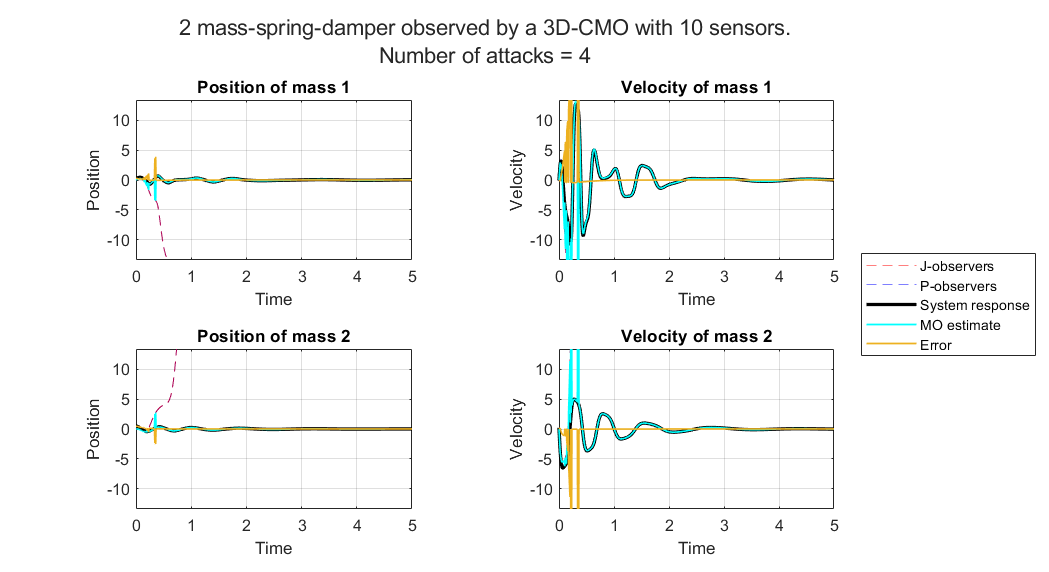
\includegraphics[width=\linewidth]{report/Figures/LAMO-attack.png}
        \caption{LAMO with $N_S=10$ and $n_{\phi}=2$, outputs 1,3,5 and 7 are under attack.}
        \label{fig:LAMO-attack}
    \end{figure}
\end{example}
